% ===============================
%       DOCUMENT CLASS
% ===============================
% Use one of the two documentclass lines depending on aspect ratio needed
% for 4x3 aspect ratio slides
% \documentclass{beamer}

% for 16x9 (modern wide screen) aspect ratio slides
\documentclass[aspectratio=169]{beamer}

% ===============================
%           PACKAGES
% ===============================
\usepackage{tikz}
\usepackage{animate}
\usepackage{tcolorbox}
\usepackage{booktabs}
\usepackage{xcolor}        % include this in your preamble
 
 
 

% ===============================
%         THEME SELECTION
% ===============================
% Oxford Maths theming
\usetheme{oxfordmaths}
 
% ===============================
%            DOCUMENT
% ===============================
\begin{document}

\setbeamercolor{background canvas}{bg=darkblue}
\begin{frame}[plain]

\color{white}
 
\vspace{0.2cm}
\centering
{\fontsize{10pt}{10pt}\selectfont\textsc{propuesta de tesis}} \\[0.1cm]
{{\fontsize{18pt}{18pt}\selectfont Aprendizaje automático en el\\[0.03cm] modelado de la propagación de ondas:}\\[0.13cm]
{\fontsize{18pt}{18pt}\selectfont De los métodos numéricos estándar a las\\[0.1cm] redes neuronales informadas por la física}} \\[0.5cm]

{\fontsize{8pt}{10pt}\selectfont
\setlength{\tabcolsep}{3pt} % antes era ~6pt
\begin{tabular}{rl}
\textbf{Estudiante:} & Oscar Rincón-Cardeño \\
\textbf{Director:} & Nicolás Guarín-Zapata, Ph.D. \\
\textbf{Codirectora:} & Silvana Montoya-Noguera, Ph.D. \\
\textbf{Grupos de investigación:} & Aplicaciones Matemáticas en Ciencias e Ingeniería \\
& Naturaleza y Ciudad \\[0.4cm]
\end{tabular}
}

{\fontsize{8pt}{10pt}\selectfont
Universidad EAFIT\\
Escuela de Ciencias Aplicadas e Ingeniería\\
Doctorado en Ingeniería\\
Noviembre de 2025\\
}

\end{frame}

\setbeamercolor{background canvas}{bg=gray!5}

\begin{frame}[plain]

\fontsize{17pt}{17pt}\selectfont\textcolor{darkblue}{Contenido}\\[0.3cm]

{\fontsize{13pt}{13pt}\selectfont
\begin{itemize} 
   \item[\raisebox{0.4ex}{\scalebox{0.7}{$\blacktriangleright$}}] Introducción\\[0.1cm]  
        
         \begin{itemize}\fontsize{12pt}{12pt}\selectfont
            \item[\raisebox{0.2ex}{\scalebox{0.5}{$\blacksquare$}}] Modelado de la propagación de ondas\\[0.1cm]
            \item[\raisebox{0.2ex}{\scalebox{0.5}{$\blacksquare$}}] Métodos numéricos estándar\\[0.1cm]
            \item[\raisebox{0.2ex}{\scalebox{0.5}{$\blacksquare$}}] Métodos basados en aprendizaje automático\\[0.2cm]
        \end{itemize}
     

    \item[\raisebox{0.4ex}{\scalebox{0.7}{$\blacktriangleright$}}] Objetivos de investigación\\[0.1cm]
    
         \begin{itemize}\fontsize{12pt}{12pt}\selectfont
            \item[\raisebox{0.2ex}{\scalebox{0.5}{$\blacksquare$}}] Objetivo general\\[0.1cm]
            \item[\raisebox{0.2ex}{\scalebox{0.5}{$\blacksquare$}}] Objetivos específicos\\[0.2cm]
        \end{itemize}    
    
    \item[\raisebox{0.4ex}{\scalebox{0.7}{$\blacktriangleright$}}] Metodología\\[0.2cm]
    \item[\raisebox{0.4ex}{\scalebox{0.7}{$\blacktriangleright$}}] Avances preliminares\\[0.2cm]      
\end{itemize}


}

\end{frame}

\setbeamercolor{background canvas}{bg=darkblue}
\begin{frame}[plain]
\addtocounter{framenumber}{-1}
 \hypertarget{Introducción}{}
 
{\huge \textcolor{white}{Introducción}}

\end{frame}


\setcounter{framenumber}{0}
\section[\raisebox{0.4ex}{\scalebox{0.7}{$\blacktriangleright$}} Introducción \hspace{0.1cm} \raisebox{0.2ex}{\scalebox{0.5}{$\blacksquare$}}\hspace{0.05cm} Modelado de la propagación de ondas]{Modelado de la propagación de ondas}



\setbeamercolor{background canvas}{bg=gray!5}
\begin{frame} 

\vspace{0.4cm}


Un \textbf{\textcolor{darkblue}{modelo matemático que describe la propagación de ondas}} en un medio en el caso directo busca representar, mediante una función, cómo evoluciona un sistema a lo largo del tiempo y en el espacio. 

\vspace{0.2cm}

\begin{figure} 
    \centering
    \includegraphics[width=0.8\textwidth]{figures/seismic_inverse_esp.pdf}
\end{figure}    

\end{frame}

\begin{frame} 

\vspace{0.8cm}

La relevancia de esta investigación se sustenta en el \textbf{\textcolor{darkblue}{creciente interés por integrar técnicas de aprendizaje automático}} en áreas tradicionalmente dominadas por métodos numéricos estándar, como la sismología.

\vspace{0.3cm}

\begin{figure} 
    \centering
    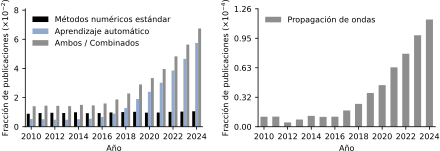
\includegraphics[width=1.0\textwidth]{figures/publication_trends_ml_wave_esp.pdf}
\end{figure}    

\end{frame}


\begin{frame} 

\vspace{0.8cm}

La investigación en aprendizaje automático fue impulsada por avances en hardware como las GPUs, un incremento significativo en la disponibilidad de datos, así como el desarrollo de \textbf{\textcolor{darkblue}{herramientas computacionales de acceso abierto}} para la implementación de estos métodos.

\vspace{0.3cm}

\begin{figure} 
    \centering
    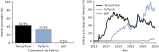
\includegraphics[width=1.0\textwidth]{figures/frameworks_esp.pdf}
\end{figure}    

\end{frame}

\begin{frame} 

Proponemos abordar la intersección entre el \textbf{\textcolor{darkblue}{aprendizaje automático}} y el modelado de \textbf{\textcolor{darkblue}{la propagación de ondas}}, específicamente en aplicaciones en \textbf{\textcolor{darkblue}{sismología}}.

\begin{figure} 
    \centering
    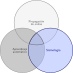
\includegraphics[width=0.45\textwidth]{figures/intersection_ml_wave_seismology_esp.pdf}
\end{figure}    

\end{frame}

\begin{frame} 

Se plantea la siguiente \textbf{\textcolor{darkblue}{pregunta de investigación}}:\\[0.5cm]

\begin{quote}
¿De qué manera el aprendizaje automático puede constituir una alternativa o un complemento para las aplicaciones relacionadas con la propagación de ondas sísmicas?
\end{quote}

\end{frame}

 
\section[\raisebox{0.4ex}{\scalebox{0.7}{$\blacktriangleright$}} Introducción \hspace{0.1cm} \raisebox{0.2ex}{\scalebox{0.5}{$\blacksquare$}}\hspace{0.05cm} Métodos numéricos estándar]{Métodos numéricos estándar}
 

%\setbeamercolor{background canvas}{bg=darkblue}
%\begin{frame}[plain]
%\addtocounter{framenumber}{-1}
% \hypertarget{Métodos numéricos estándar}{}
% 
%{\huge \textcolor{white}{Métodos numéricos estándar}}
%
%\end{frame}

\setbeamercolor{background canvas}{bg=gray!5}
\begin{frame} 

En los \textbf{\textcolor{darkblue}{métodos numéricos estándar}} la precisión requerida que se logra depende de la discretización de la malla computacional.

\vspace{0.3cm}

\begin{figure} 
    \centering
    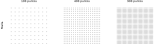
\includegraphics[width=1.0\textwidth]{figures/mallas.pdf}
\end{figure}    

\end{frame}

\begin{frame} 

Consideremos \textbf{\textcolor{darkblue}{el caso de la solución aproximada $\boldsymbol{\hat{f}}$ obtenida mediante el método de diferencias finitas}} para la ecuación de Helmholtz:
 
\begin{equation*}
\begin{cases}
\nabla^2 f + (5\pi)^2 f = 0, & \text{en } \Omega, \\[6pt]
f = 0, & \text{en } \partial\Omega.
\end{cases}
\end{equation*}

\indent La solución analítica correspondiente está dada por

\[
f(x,y) = \sin(5\pi x)\sin(5\pi y).
\]
    
\end{frame}

\begin{frame} 

El refinamiento de la malla mejora la aproximación numérica.

\vspace{0.3cm}

\begin{figure} 
    \centering
    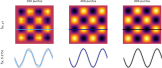
\includegraphics[width=1.0\textwidth]{figures/solucion_diferencias_finitas.pdf}
\end{figure} 

\end{frame}

\begin{frame} 

Se reduce el error relativo con respecto a la solución analítica y, al mismo tiempo, incrementa el tiempo de cómputo.

\vspace{0.3cm}

\begin{figure} 
    \centering
    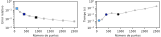
\includegraphics[width=1.0\textwidth]{figures/convergencia.pdf}
\end{figure} 

\end{frame}

 

\section[\raisebox{0.4ex}{\scalebox{0.7}{$\blacktriangleright$}} Introducción \hspace{0.1cm} \raisebox{0.2ex}{\scalebox{0.5}{$\blacksquare$}}\hspace{0.05cm} Métodos basados en aprendizaje automático]{Métodos basados en aprendizaje automático}

%\setbeamercolor{background canvas}{bg=darkblue}
%\begin{frame}[plain]
%\addtocounter{framenumber}{-1}
% \hypertarget{Métodos basados en aprendizaje automático}{}
% 
%{\huge \textcolor{white}{Métodos basados en aprendizaje automático}}
%
%\end{frame}

\setbeamercolor{background canvas}{bg=gray!5}

\begin{frame}{Aprendizaje automático como alternativa para el modelado de la propagación de ondas} 

\end{frame}

\begin{frame}{¿Qué es una red neuronal?} 
 
Una red neuronal puede entenderse como una función \(f(x)\) que es 
\textbf{\textcolor{darkblue}{la composición de varias funciones}} \(g_i(x)\), 
cada una de las cuales aplica una transformación a la entrada \(x\):
\[
f(x) = g_n(g_{n-1}(\ldots g_2(g_1(x))\ldots)).
\]

Cada función \(g_i(x)\) puede escribirse como:
\[
g_i(x) = \sigma(w_i x + b_i),
\]
donde \(w_i\) y \(b_i\) son parámetros ajustables (peso y sesgo, respectivamente), y \(\sigma\) es una función de activación no lineal.    

\end{frame}



\begin{frame}{Teorema de aproximación universal}

\begin{quote}
Una red neuronal con una sola capa oculta y cierto número finito de neuronas puede aproximar de manera arbitraria cualquier función continua, dada una función de activación adecuada.
\end{quote}


\begin{figure} 
    \centering
    
\includegraphics[width=1.0\textwidth]{figures/universal_approximation_nn.pdf}
\end{figure} 

\end{frame}

\begin{frame}{Ejemplo: aproximación de funciones con redes neuronales}

Queremos aproximar la siguiente función:
\[
f(x) = x^3 + x^2 - x - 1.
\]
Utilizando una red neuronal de una sola capa de la forma:
\[
f(x) \approx \hat{f}_{i}(x) = \sum_{i=1}^{N} g_i(x).
\]
donde cada función $g_i(x)$ está dada por:
\[
g_i(x) = w_i \, \text{ReLU}(x - x_i^*) + y^{\text{offset}}_{i}.
\]

\end{frame}


\begin{frame} 
\begin{figure} 
    \centering
    
\includegraphics[width=1.0\textwidth]{figures/universal_approximation_demo_net.pdf}
\end{figure} 

\end{frame}

\begin{frame} 
\begin{figure} 
    \centering
    \includegraphics[width=1.0\textwidth]{figures/universal_approximation_demo_plot.pdf}
\end{figure} 

\end{frame}

\begin{frame} 

\begin{quote}
Aunque una red de una sola capa es capaz de aproximar cualquier función, dicha capa podría requerir un número de neuronas inviable y aun así no garantizar un aprendizaje y generalización adecuados.
\end{quote}

\end{frame}

\begin{frame} 
\begin{figure} 
    \centering
    \includegraphics[width=1.0\textwidth]{figures/scheme_surrgate_models_NNs_esp.pdf}
\end{figure} 

\end{frame}


\begin{frame} 
\begin{figure} 
    \centering
    \includegraphics[width=1.0\textwidth]{figures/scheme_PINNs_esp.pdf}
\end{figure} 

\end{frame}

\begin{frame} 
\begin{figure} 
    \centering
    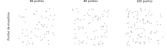
\includegraphics[width=1.0\textwidth]{figures/pinn_sampling_esp.pdf}
\end{figure} 

\end{frame}


\begin{frame} 
\begin{figure} 
    \centering
    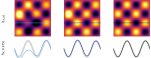
\includegraphics[width=1.0\textwidth]{figures/pinn_approximation_demo.pdf}
\end{figure} 

\end{frame}

\begin{frame} 
\begin{figure} 
    \centering
    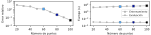
\includegraphics[width=1.0\textwidth]{figures/pinn_convergence_demo.pdf}
\end{figure} 

\end{frame}


\section[\raisebox{0.4ex}{\scalebox{0.7}{$\blacktriangleright$}} Objetivos de la investigación \hspace{0.1cm} \raisebox{0.2ex}{\scalebox{0.5}{$\blacksquare$}}\hspace{0.05cm} Objetivo general]{Objetivo general}


\setbeamercolor{background canvas}{bg=darkblue}
\begin{frame}[plain]
\addtocounter{framenumber}{-1}
 \hypertarget{Objetivos de investigación}{}
 
{\huge \textcolor{white}{Objetivos de investigación}}

\end{frame}

\setbeamercolor{background canvas}{bg=gray!5}
\begin{frame}

\textbf{\textcolor{darkblue}{Objetivo general:}}\\[0.4cm]

Desarrollar enfoques de aprendizaje automático que puedan constituir una alternativa o complemento a los métodos numéricos estándar en la modelación de la propagación de ondas, con énfasis en la evaluación de su rendimiento computacional y aplicabilidad en sismología.

\end{frame} 


\section[\raisebox{0.4ex}{\scalebox{0.7}{$\blacktriangleright$}} Objetivos de la investigación \hspace{0.1cm} \raisebox{0.2ex}{\scalebox{0.5}{$\blacksquare$}}\hspace{0.05cm} Objetivos específicos]{Objetivos específicos}

\begin{frame}
 
\textbf{\textcolor{darkblue}{Objetivos específicos:}}\\[0.4cm]

{\fontsize{10pt}{10pt}\selectfont 
\begin{itemize}
     \item \textbf{\textcolor{darkblue}{Mapear}} las técnicas de aprendizaje automático utilizadas en el modelado de la ecuación de ondas aplicadas a la sismología, resaltando sus aplicaciones, alcances y desafíos actuales.
     \item \textbf{\textcolor{darkblue}{Comparar}} métodos representativos de aprendizaje automático, frente a enfoques numéricos estándares, evaluando su precisión y eficiencia computacional, destacando sus ventajas, limitaciones y potencial de integración.
     \item \textbf{\textcolor{darkblue}{Evaluar}} la capacidad de las PINNs para resolver problemas inversos en sismología, en lo referente a mantener una precisión comparable a la de los métodos estándar y, al mismo tiempo, reducir los costos computacionales.
     \item \textbf{\textcolor{darkblue}{Escalar}} los enfoques basados en aprendizaje automático para favorecer el uso de datos provenientes de problemas en sismología en escenarios no controlados.
\end{itemize}
}

\end{frame}


\begin{frame}

\begin{figure} 
    \centering
    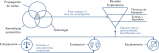
\includegraphics[width=1.0\textwidth]{figures/escheme_objetives.pdf}
\end{figure} 

\end{frame}


\section[\raisebox{0.4ex}{\scalebox{0.7}{$\blacktriangleright$}} Métodología]{Métodología}

\setbeamercolor{background canvas}{bg=darkblue}
\begin{frame}[plain]
\addtocounter{framenumber}{-1}
 \hypertarget{Métodología}{}
 
{\huge \textcolor{white}{Métodología}}

\end{frame}

\setbeamercolor{background canvas}{bg=gray!5}

\begin{frame}
\begin{figure} 
    \centering
    \includegraphics[width=1.0\textwidth]{figures/methodology.pdf}
\end{figure} 

\end{frame}


 
\section[\raisebox{0.4ex}{\scalebox{0.7}{$\blacktriangleright$}} Avances preliminares]{Avances preliminares}

\setbeamercolor{background canvas}{bg=darkblue}
\begin{frame}[plain]
\addtocounter{framenumber}{-1}
 \hypertarget{Avances preliminares}{}
 
{\huge \textcolor{white}{Avances preliminares}}

\end{frame}

\setbeamercolor{background canvas}{bg=gray!5}
\begin{frame} 
 
\end{frame}
 

\setbeamercolor{background canvas}{bg=gray!5}
\begin{frame} 

 

\begin{quote}
¿Cómo pueden compararse los enfoques modernos basados en aprendizaje automático para resolver PDEs con los métodos numéricos estándar?
\end{quote}
 
\end{frame}

\begin{frame} 
 
\end{frame}

\begin{frame} 
 
\end{frame}

\begin{frame} 
 
\end{frame}

\setbeamercolor{background canvas}{bg=darkblue}
\begin{frame}[plain]

\textcolor{white}{\textbf{Contacto:} orincon@eafit.edu.co}\\
  
 


\end{frame}

\end{document}
